\documentclass[9pt,a4paper,twoside]{tau}
\usepackage[english]{babel}
\usepackage{tauenvs}

%----------------------------------------------------------
% TITLE
%----------------------------------------------------------

\title{Energy Transfer Stock Analysis and Investment Potential: A Comprehensive Report}

%----------------------------------------------------------
% AUTHORS, AFFILIATIONS AND PROFESSOR
%----------------------------------------------------------

\author[a,1]{Justin Bucsa}
\author[b,2]{Sunrit Sarkar}
\author[b,c,3]{Hassan Attarchi, PhD}

%----------------------------------------------------------

\affil[a]{Stealth}
\affil[b]{Stealth}
\affil[c]{Stealth \& University of California, Riverside}



%----------------------------------------------------------
% FOOTER INFORMATION
%----------------------------------------------------------

\institution{Stealth}
\ftitle{\LaTeX\ Template}
\date{June 27, 2024}
\etal{Bucsa}


%----------------------------------------------------------
% ABSTRACT
%----------------------------------------------------------

\begin{abstract}    
    This report analyzes the short-term and long-term investment potential of Energy Transfer (ET) stock by examining its business model, recent events, competitive landscape, and financial performance. Quantitative models, including Volume Weighted Average Price (VWAP), linear regression, Bollinger Bands, and Autoregressive Integrated Moving Average (ARIMA), are employed to assess the stock's valuation and forecast potential price movements. The analysis reveals a complex picture, with indicators suggesting short-term overvaluation and potential price correction, while long-term prospects remain uncertain due to challenges in revenue growth and industry competition. The report concludes with recommendations for both short-term and long-term investment strategies. 
\end{abstract}

%----------------------------------------------------------

\keywords{Energy Transfer [ET], VMAP, Linear Regression, Bollinger Band, ARIMA}

%----------------------------------------------------------

\begin{document}
		
	\maketitle
	\thispagestyle{firststyle}
	\tauabstract
	\tableofcontents

%----------------------------------------------------------

\section{Introduction}

    Energy Transfer LP (ET) is a leading energy infrastructure company specializing in transporting and storing natural gas, natural gas liquids (NGLs), crude oil, and refined products. With a vast network of pipelines, terminals, and processing facilities across the United States, ET plays a crucial role in the energy sector. This report aims to assess the investment potential of ET stock in both the short-term and long-term horizons.

    The analysis will delve into ET's business model, recent events, competitive landscape, and financial performance. To provide a comprehensive evaluation, we will employ various quantitative models, including Volume Weighted Average Price (VWAP), linear regression, Bollinger Bands, and Autoregressive Integrated Moving Average (ARIMA). These models will help us gauge the stock's current valuation, predict potential price movements, and assess its overall attractiveness for investors.
    
    By examining fundamental and technical factors, this report seeks to offer valuable insights to investors considering ET as a potential addition to their portfolios. Whether you are a short-term trader seeking quick gains or a long-term investor looking for stable returns, this report will provide a balanced assessment of ET's investment potential and recommendations tailored to different investment strategies.


\section{What is Energy Transfer}
    Energy Transfer LP operates as a diversified energy partnership, primarily focused on the midstream sector of the oil and gas industry. 

    \subsection{Business Model}
        Their business model revolves around owning and operating a vast network of energy infrastructure assets across the United States. These assets include:
        
        - Intrastate and Interstate Pipelines: Energy Transfer owns and operates an extensive network of natural gas pipelines, both intrastate (within a single state) and interstate (across multiple states). These pipelines transport natural gas from production areas to various markets, including industrial consumers, utilities, and power generators\cite{energy-transfer-2024}.
        
        - Storage Facilities: The partnership also owns and operates natural gas storage facilities, allowing them to store natural gas during periods of low demand and release it during peak demand, thereby optimizing the utilization of their pipeline network and generating additional revenue\cite{energy-transfer-2024}.
        
        - Midstream Operations: Energy Transfer's midstream operations encompass a wide range of activities, including natural gas gathering, processing, treating, and transportation. They own and operate processing plants, treating facilities, and gathering systems in major producing basins across the country\cite{energy-transfer-2024}.
        
        - NGL and Refined Products Transportation and Services: The partnership is involved in the transportation, storage, and fractionation of natural gas liquids (NGLs) and refined products. They own NGL pipelines, fractionation facilities, and terminals, enabling them to participate in the NGL value chain from production to market\cite{energy-transfer-2024}.
        
        - Crude Oil Transportation and Services: Energy Transfer also owns and operates crude oil pipelines and terminals, providing transportation and storage services for crude oil producers and refiners. They have a significant presence in major crude oil producing regions, including the Permian Basin\cite{energy-transfer-2024}.
        
        - Investments in Sunoco LP and USAC: Energy Transfer holds investments in two master limited partnerships (MLPs): Sunoco LP, which is primarily engaged in fuel distribution and marketing, and USAC, which provides natural gas compression services. These investments contribute to Energy Transfer's diversified income stream\cite{energy-transfer-2024}.


    \subsection{Business Strategy}
    
        Energy Transfer's business strategy is centered around several key pillars:
        
        1. Growth through Acquisitions: The partnership actively pursues strategic acquisitions of assets and businesses that complement its existing portfolio and offer opportunities for operational synergies and increased utilization of its infrastructure\cite{energy-transfer-2024}.
        
        2. Organic Growth Projects: Energy Transfer invests in the construction and expansion of its existing systems to meet growing demand for midstream and transportation services. This includes building new pipelines, expanding processing capacity, and developing new storage facilities\cite{energy-transfer-2024}.
        
        3. Fee-Based Revenue: The partnership aims to increase the proportion of its revenue generated from fee-based contracts, which provide stable and predictable cash flows compared to commodity-based revenues. This is achieved by securing long-term contracts with customers for transportation, storage, and processing services\cite{energy-transfer-2024}.
        
        4. Profitability Enhancement: Energy Transfer focuses on enhancing the profitability of its existing assets by optimizing operations, reducing costs, and increasing throughput volumes\cite{energy-transfer-2024}.

    \subsection{Financial Performance}
    
        ET's financial performance is primarily driven by the cash distributions it receives from its subsidiaries, including Sunoco LP and USAC. The partnership's revenue streams are diversified across various segments, with a significant portion coming from fee-based contracts. However, the partnership is also exposed to commodity price fluctuations, which can impact its profitability\cite{energy-transfer-2024}.
    
    \subsection{Summary of Energy Transfer}
        
        Overall, ET's business model is characterized by its extensive energy infrastructure network, diversified revenue streams, and focus on growth through acquisitions and organic projects. The partnership's strategy of increasing fee-based revenue and optimizing existing assets aims to provide stable cash flows and long-term value for its unit holders.


\section{Recent Major Events}
    
    This section will discuss events that may or may not have impacted share prices over the last two years but are still worth mentioning. 
    
    - December 2022 - An explosion occurred at Energy Transfer's Revolution Cryo plant in Smith Township, Washington County, Pennsylvania. The blast was caused by a defective valve that released a vapor cloud of natural gas liquids, which then ignited. While no injuries were reported, the incident led to an investigation by the Pennsylvania Department of Environmental Protection (DEP) \cite{commonwealth-of-pennsylvania-department-of-environmental-protection-air-quality-program-2023} \cite{energy-transfer-2024}.


\section{Competitors}
    
    Energy Transfer (ET) has several top competitors in the energy sector, primarily in the midstream space. Some of the most notable competitors include:
    
    - Kinder Morgan (KMI): One of the largest energy infrastructure companies in North America, operating a vast network of pipelines and terminals \cite{seeking-alpha-no-date} \cite{tracxn-technologies-limited-no-date}.
    
    - Enterprise Products Partners (EPD): A leading midstream energy company with a diversified asset base, including pipelines, storage facilities, and processing plants \cite{seeking-alpha-no-date}.
      
    - Williams Companies (WMB): A large natural gas infrastructure company with significant gathering and processing operations \cite{seeking-alpha-no-date}.
    
    - ONEOK (OKE): A major player in the natural gas liquids (NGL) market, with a focus on NGL gathering, fractionation, transportation, and storage \cite{seeking-alpha-no-date}.
    
    - Plains All American Pipeline (PAA): A leading transporter of crude oil and NGLs, primarily in North America \cite{craftco-no-date}.
    
    - Targa Resources (TRGP): A diversified midstream energy company with natural gas gathering and processing assets, NGL fractionation and transportation, and crude oil gathering and terminaling \cite{craftco-no-date}.\\
    
    These are just a few of Energy Transfer's top competitors. The competitive landscape can vary depending on the specific market and segment within the energy industry.

    \subsection{Analysis}
    
        Observing the closing price of ET stock and its competitors over the last two years reveals some significant differences (see Figure 1). 
    
        1. ET stock has grown slightly over the last two years with limited volatility.

        2. All competitors showed positive growth over the last two years.

        3. ET has grown the least out of all the competitors.

        
        \begin{figure}[H]
            \centering
            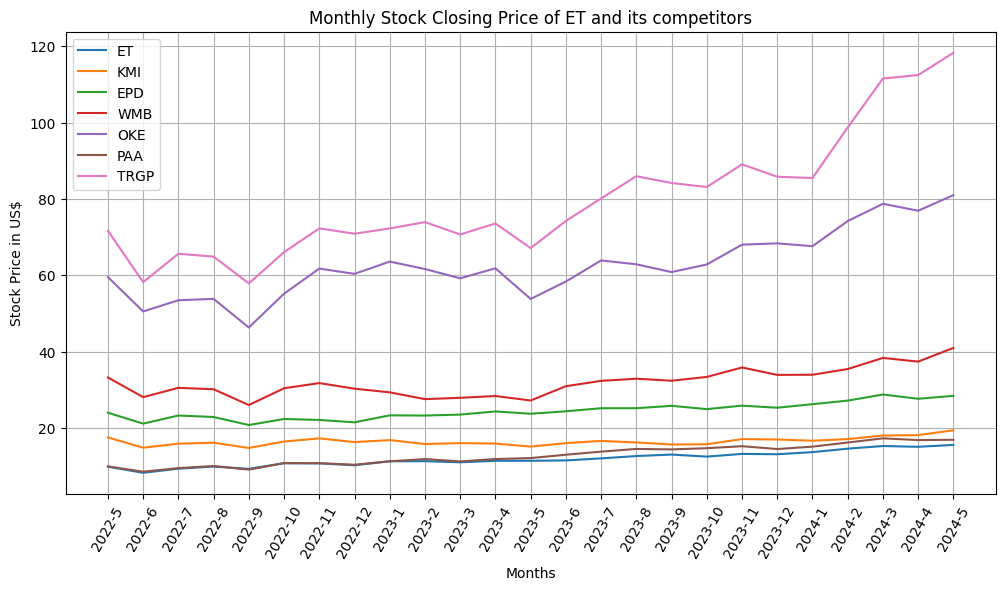
\includegraphics[width=0.85\columnwidth]{Figures/MonthlyStockClosingPrices.png}
            \caption{This chart shows the monthly closing price for the last two years between ET and similar competitors\cite{yahoo-finance-2024}.}
            \label{fig:figure}
        \end{figure}
        
        \subsubsection{Conclusion}
        
            Although ET has shown positive growth within the last two years, this may be more due to the overall industry conditions than to ET's performance as a company. Therefore, ET is a safe financial investment in the short term (1 month to 6 months), but due to its competitive landscape, it may be a better investment in the long term (1 year and plus).

\section{Review of Quarterly Reports}

    This section will discuss ET's quarterly revenue over the past two years and assess its short-term and long-term impact on the stock price.

    The line graphs below in figure 2 reflect the quarterly revenue, net income, adjusted EBITDA, and earnings per share over the last two years for ET.

    \begin{figure}[H]
        \centering
        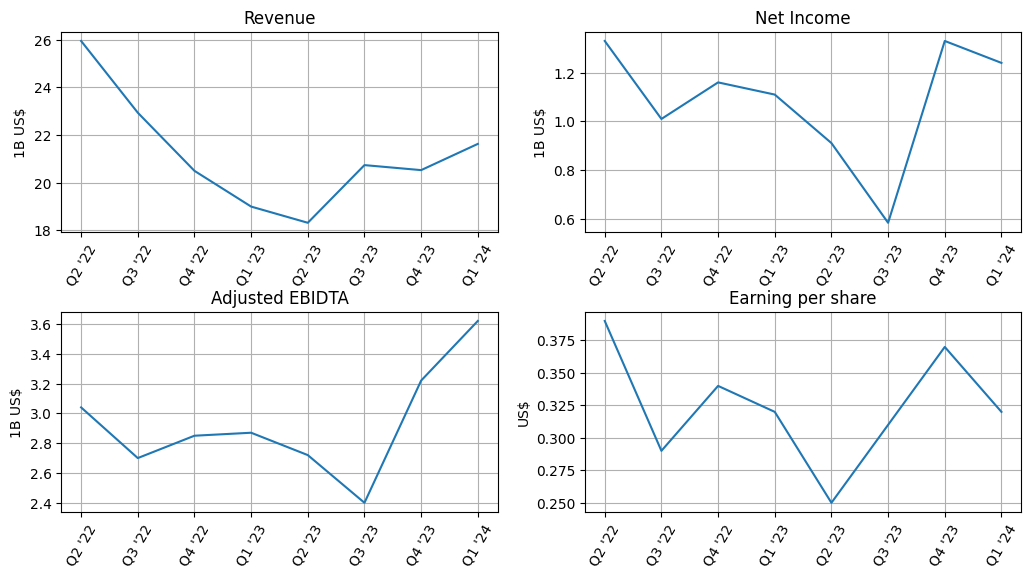
\includegraphics[width=0.85\columnwidth]{Figures/Revenue_NetIncome_AdjustedEBIDTA_GAAPearningPerShare.png}
        \caption{Four line graphs that reflect the quarterly revenue, net income, adjusted EBITDA, and earnings per share over the last two years for Energy Transfer [ET]\cite{alpha-vantage-2024}.}
        \label{fig:figure}            
    \end{figure}

    Notably, ET's revenue peaked over two years ago. To compensate for the loss in revenue, ET has focused its resources on reducing overhead costs.

    The reduction in overhead costs has positively impacted ET's EBITDA, reaching its highest level in the past two years. This suggests a company cutting costs as income levels decrease. However, it's alarming that even with the highest EBITDA in two years, the earnings per share value is still decreasing, indicating that investors anticipate a decrease in EBITDA returns in the near future.

    \subsection{Conclusion}

    After reviewing ET's quarterly revenue, net income, adjusted EBITDA, and earnings per share over the last two years, the conclusion is that a loss is unavoidable. ET can only cut overhead costs gradually, as they must meet operational standards to avoid potential closure by federal and local governments.

    It is logical to believe that ET could maintain its current level of net income. This means that its stock value will drop in the short term, but this could be a necessary readjustment to the price, as noted in the section on the VWAP model, which indicates that the stock is trading well above its value. Therefore, based on the current analysis, ET is not a good investment for the next six months to a year.
    
    If the price can reset at a lower rate, it may still become an ideal, more prolonged investment, but the returns may still be minor compared to industry standards like the S\&P 500.

\section{Impact of Trade Volume}

    This section will cover the trading volume of ET stock, compare it to competitors' trading volume, and conclude its impact on the short-term and long-term investment analysis.

    The bar chart in Figure 3 illustrating the monthly traded volume of ET stock over the past two years reveals a drastic change since May 2022. The current trading volume of ET is almost 50\% of the volume traded in May 2022. This indicates a decrease in the number of individuals willing to trade ET stock. 
    
    \begin{figure}[H]
        \centering
        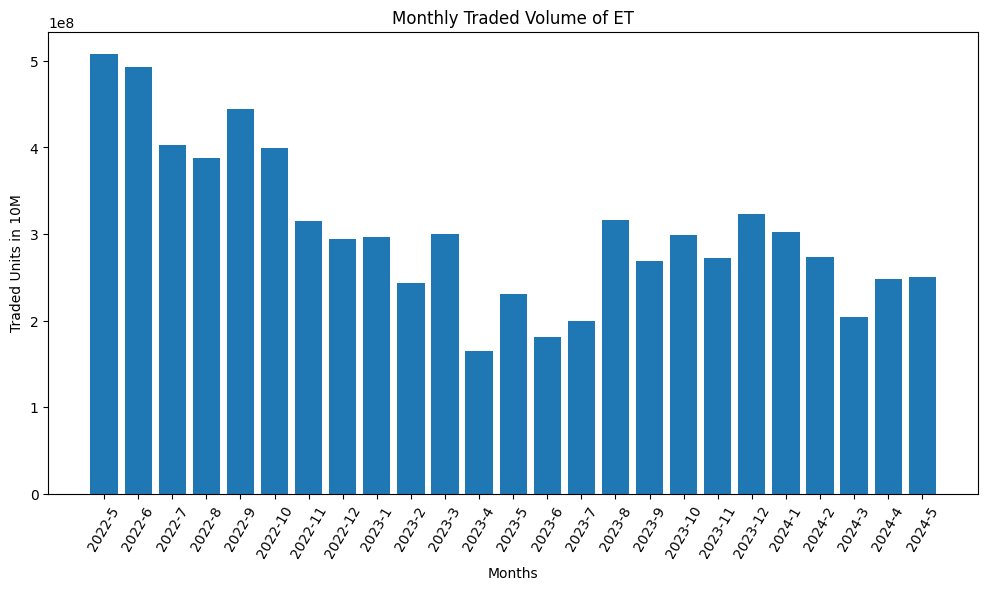
\includegraphics[width=0.85\columnwidth]{Figures/MonthlyTradedVolumeOfET.png}
        \caption{Bar chart shows the monthly Trading volume of Energy Transfer [ET] stock over the past two year\cite{yahoo-finance-2024}.}
        \label{fig:figure}
    \end{figure}

    When ET's trading volume is compared to its competitors', we find that ET and Kinder Morgan (KMI) have lower stock prices and potentially higher trading volumes (see figure 4). Competitors with higher stock prices generally trade at lower volumes. When considering both volume and price, all companies within this industry trade at a balanced weight.

    \begin{figure}[H]
        \centering
        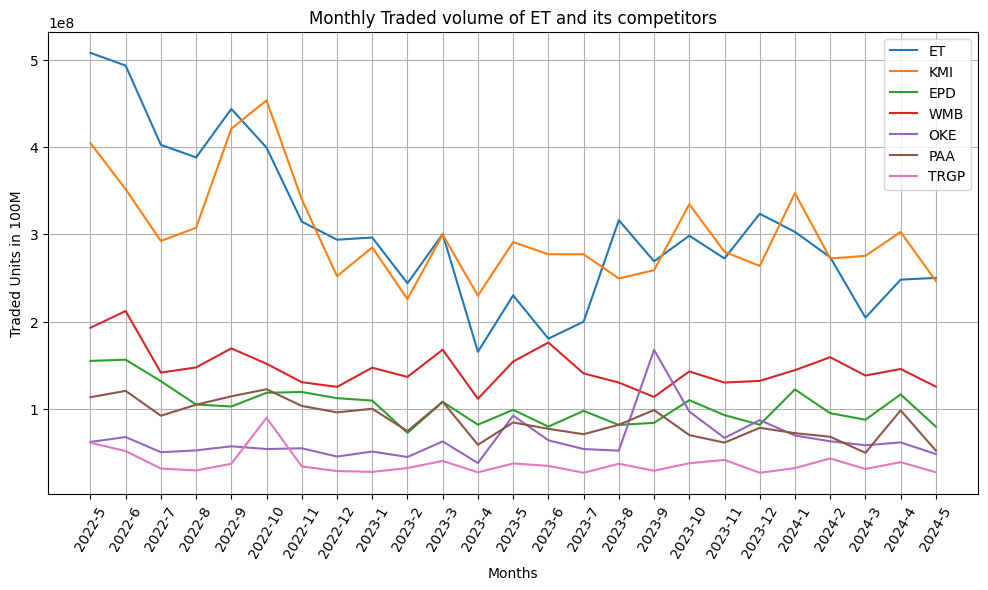
\includegraphics[width=0.85\columnwidth]{Figures/MonthlyTradedVolumeOfETvsCompetitors.png}
        \caption{This line graph shows the monthly trading volume of ET stock and its competitors for the last two years\cite{yahoo-finance-2024}.}
        \label{fig:figure}
    \end{figure}

    An interesting observation is that Targa Resources (TRGP) and ONEOK (OKE) trade volumes have remained relatively stable, with only a few spikes before returning to normal levels. Notably, their stock prices have steadily increased to a two-year maximum. This trend may suggest the superiority of OKE and TRGP as investments compared to ET.end, which may uglier the superiority of OKE and TRGP as an investment over ET. 

    \subsection{Conclusion}

        The analysis of ET's trading volume history over the past two years reveals the following: 
        
        1. The trading volume of ET stock is continually decreasing.

        2. ET stock volume is 200\% to 300\% higher than its competitors, except for KMI.
        
        3. There is a balance among all competitors when considering stock volume and price.
        
        Therefore, we can conclude that the industry is performing well, but only some companies are clear leaders. The data in this section needs to provide a definitive answer on whether ET is an ideal long-term or short-term investment. 
        


\section{Quantitative Models}

    This section will discuss ET's performance when evaluated against quantitative modeling techniques. Please take a look at the Appendix for more explanation of the mathematics behind each model.

    \subsection{VMAP Model}
    
        The VWAP model, created from ET's closing price over the last two years, is shown below. VWAP is commonly used as a reference point for traders and investors to assess the execution price of their orders. Selling above VWAP is considered advantageous, implying a higher price than the average. ET has been trading well above its VWAP value.

        \begin{figure}[H]
            \centering
            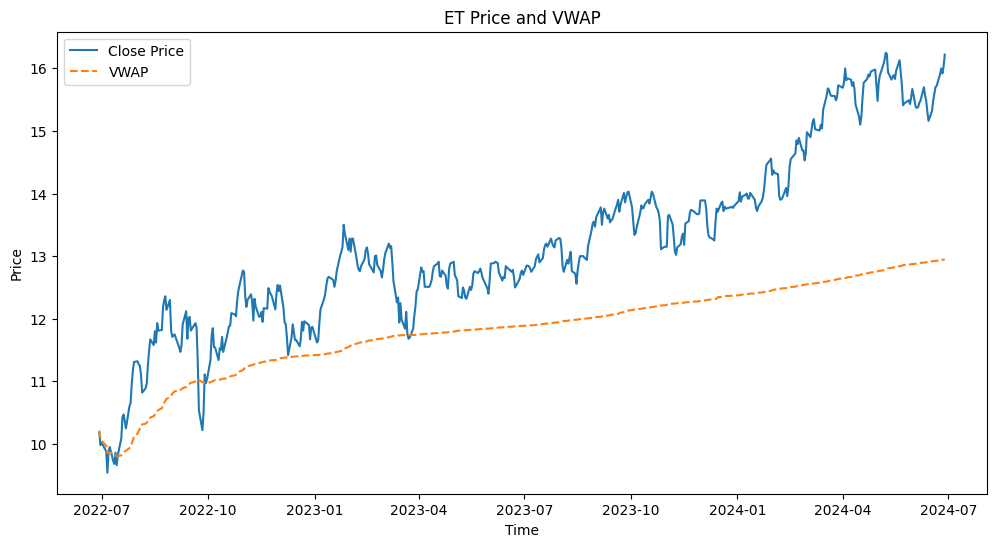
\includegraphics[width=0.85\columnwidth]{Figures/ETPriceAndVWAP.png}
            \caption{This chart is the VMAP model based on the closing price of Energy Transfer [ET] stock from the last two years\cite{yahoo-finance-2024}.}
            \label{fig:figure}
        \end{figure}

        This leads to the acknowledgment that ET is trading at a significantly overvalued price. This implies that a price correction is due it is coming in the near future. 

        \subsubsection{Conclusion}
        
            ET has been trading well above its VWAP for over a year, signaling a potential correction of 25\% to meet the VWAP price. This implies high volatility in ET stock. The price may only be supported due to the nature of the industry, as noted in the "Competitors" section. Thus, the VWAP model suggests that ET is not wise for long-term or short-term investments.

    \subsection{Linear Regression Model}
    
        This section discusses the linear regression trend line of the stock value for the last two years.\\

        Figure 6 shows the resulting linear regression trend line related to ET's closing prices over the past two years. The positive slope indicates a positive return from an investment in ET over the past two years. This can be used to predict a positive return in the short term but is unreliable for predictions beyond a few weeks to a few months.

    
        \begin{figure}[H]
            \centering
            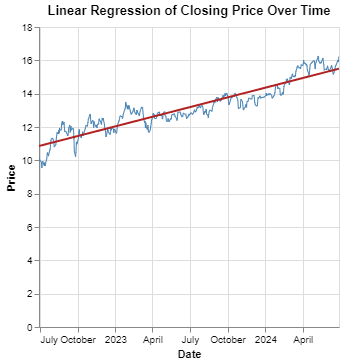
\includegraphics[height=.50\columnwidth]{Figures/LinearRegression.png}
            \caption{This graph shows the Linear Regression trend line against the Closing Stock Price of ET over the past two years\cite{yahoo-finance-2024}.}
            \label{fig:figure}
        \end{figure}  
        
        \subsubsection{Conclusion}

        The linear regression model provides positive information supporting investment in ET. However, it's important to note that it's not designed for long-term predictions but only for the limited short term.

        Therefore, we can conclude that day trading ET stock may be profitable for the next few months, but we cannot draw any positive conclusions for long-term investment.

    \subsection{Bollinger Band Model}

        Applying the Bollinger Band model to ET's historical closing price over the past two years helps identify potential overbought and oversold conditions and potential trend reversals. Figure 7 represents the Bollinger Band model applied to ET's historical closing price. The figure clearly shows that ET's stock price is trading above the upper band, indicating overpriced. It's important to note that the stock price has been trading near the upper band since April 2023.

        \begin{figure}[H]
            \centering
            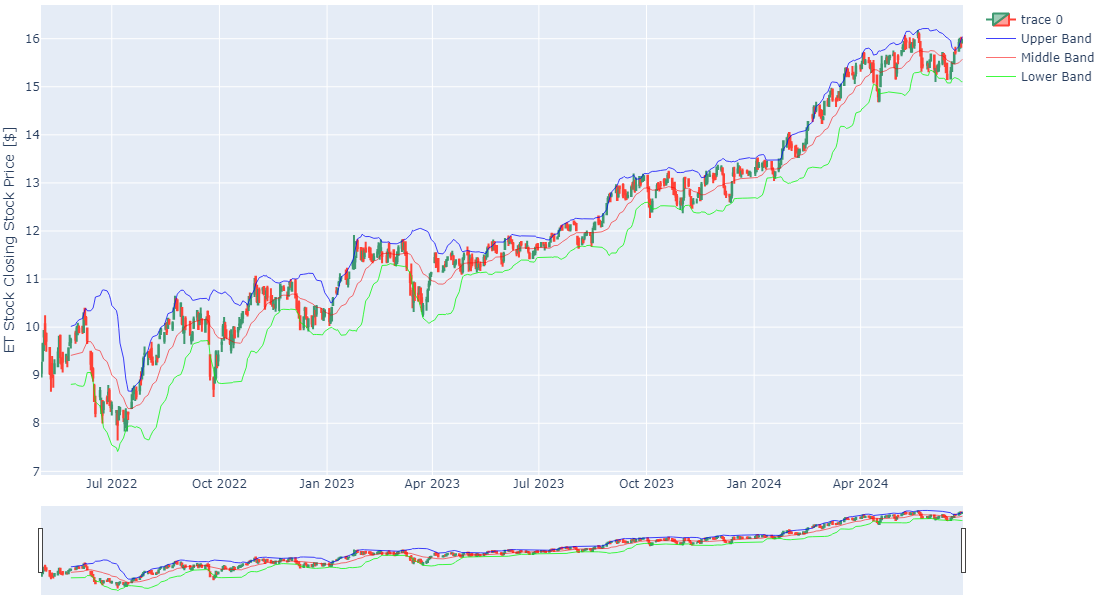
\includegraphics[width=0.85\columnwidth]{Figures/Bollinger_Bands.png}
            \caption{This figure captures the Bollinger Band models for based upon closing prices from the last two years\cite{yahoo-finance-2024}.}
            \label{fig:figure}
        \end{figure}

        \subsubsection{Conclusion}

            The Bollinger Band model shows that ET stock has been trading at the upper band for over a year. This indicates that the stock price is nearing a correction period leading to a fall. Due to this, ET is not an ideal short-term investment because of the negative impacts of the coming price correction.

            As for long-term investment, it's difficult to determine if the Bollinger Band model can predict any positive or negative future for ET's stock price. Therefore, we cannot rely on the Bollinger Band model to assist in this analysis for a long-term investment in ET stock.

    \subsection{ARIMA Model}
    
        The ARIMA (Autoregressive Integrated Moving Average) model is a statistical method widely used for analyzing and forecasting time series data, including stock prices. Figure 8 uses the ARIMA model to predict ET's future stock price for the next 30 days. 
        
        \begin{figure}[H]
            \centering
            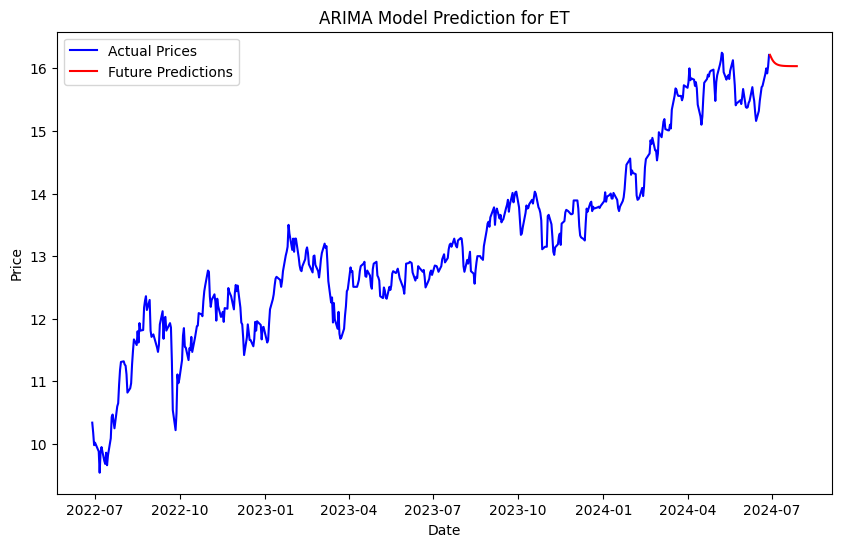
\includegraphics[width=0.85\columnwidth]{Figures/ARIMA_ModelPredictionET.png}
            \caption{Example \cite{yahoo-finance-2024}.}
            \label{fig:figure}
        \end{figure}

        As seen in Figure 8, the ARIMA model predicts a negative forecast for ET's price in the near future. This may be the start of the price correction noted in section 7.3 (Bollinger Band Model).

            \subsubsection{Conclusion}

                The ARIMA model concludes that ET's price will fall shortly. Thus, ET is not a wise short-term investment. However, ET may be a wise long-term investment after the predicted stock price drop 

\section{Overall Conclusion}

    After analyzing the data and applying various quantitative models, a few critical insights emerge regarding ET's investment potential: 

    \subsection{Short-Term Outlook}

        The VWAP, Bollinger Bands, and ARIMA models all suggest a potential price correction in the short term. Given the current overvaluation and declining trading volume, ET may not be a suitable investment for short-term gains over the next few months to a year. 

    \subsection{Long-Term Outlook}

        While the linear regression model suggests a positive trend over the past two years, it's unreliable for long-term forecasting. The declining revenue and competitive landscape raise concerns about ET's long-term growth prospects. However, the recent EBITDA and cost management improvements could signal a potential turnaround, making ET a potential long-term investment after the price correction. 

\section{Recommendations}

    Based on the analysis presented in this report, here are our recommendations for different investment strategies:

    \subsection{Short-Term Investors}

        Given the expected price correction, avoiding investing in ET for short-term gains is advisable. Potential investors should wait for the stock price to stabilize and show signs of a reversal before considering a short-term position.

    \subsection{Long-Term Investors}

        For long-term investors, the outlook is more nuanced. While the company faces challenges, the recent improvements in operational efficiency and potential for price correction present a possible buying opportunity. However, thorough due diligence is crucial, including closely monitoring industry trends, competitor performance, and ET's financial results in subsequent quarters. If ET can sustain its cost-cutting measures and demonstrate revenue growth, it could become an attractive long-term investment option.

\section{Disclaimer}

    This report is intended for informational purposes only and should not be considered financial advice. The analysis and conclusions presented are based on historical data and quantitative models, which have inherent limitations. Investing in the stock market carries risks, and past performance is not indicative of future results. Investors should always conduct their own research and consult with a financial advisor before making any investment decisions.

\section{Appendix}

    This Appendix section reviews the mathematical models used to analyze and forecast the stock prices within this report.

    \subsection{VWAP Model}

        The Volume Weighted Average Price (VWAP) is a trading benchmark calculated as the ratio of the total value traded to the total volume traded over a specific time period (typically a trading day).
    
        \begin{equation}
        VWAP = (\sum_{i=1}^{n} (P_i * V_i)) / ((\sum_{i=1}^{n} V_i)
        \end{equation}
            where:
        \begin{align}
        \text{range is i &= 1 to n}\\
        \end{align}


    \subsection{Linear Regression}

        Linear regression models the relationship between a dependent variable and one or more independent variables. The following is a simple linear model with time as the independent variable:

        \begin{equation}
        P_t = \alpha + \beta t + \epsilon_t
        \end{equation}
        
        where:
        \begin{align*}
        P_t &= \text{the stock price at time, t}\\
        \alpha &= \text{the intercept (the price when $t =0$)}\\
        \beta &= \text{the slope (the rate of price change over time)}\\
        \epsilon_ &= \text{the error term representing random fluctuations}\\
        \end{align*}  
        
        We'll fit this model to historical ET price data to estimate $\epsilon$ and $\beta$. This can provide a baseline understanding of the stock's price trend over time, but it may not capture more complex patterns.




    \subsection{ARIMA (Autoregressive Integrated Moving Average)}
        
        ARIMA models are more sophisticated and designed for time series data like stock prices. They combine three components:\\
        
        Autoregression (AR): Models the relationship between a current value and its past values.
        
        Differencing (I): Makes the time series stationary (i.e., removes trends and seasonality).
        
        Moving Average (MA): Models the relationship between a current value and past forecast errors.\\
        
        
        A general ARIMA(p,d,q) model is represented as:
        
        \begin{equation}
        (1 - \phi_1B - \dots - \phi_pB^p)(1-B)^d X_t = (1 + \theta_1B + \dots + \theta_qB^q) \epsilon_t
        \end{equation}
        
        where:
        \begin{align*}
        X_t &= \text{the differenced time series}\\
        B &= \text{the backshift operator (e.g., $BX_t=X_(t−1)$)}\\
        p &= \text{the order parameters for AR}\\
        d &= \text{the order parameters for I}\\
        q &= \text{the order parameters for MA}\\
        \phi_1,  \dots ,  \phi_P &= \text{the autoregressive coefficients}\\
        \theta_1,  \dots ,  \theta_P &= \text{the moving average coefficients}\\
        \end{align*}  
           
         Typically, a statistical technique is used to determine the best values of p, d, and q based on shock data. ARIMA can capture more complex patterns and dependencies within the time series, potentially providing more accurate forecasts than simple linear regression.

    \subsection{Bollinger Bands: A Dynamic Measure of Volatility and Potential Trading Signals}
    
        Bollinger Bands are a popular technical analysis tool used to assess price volatility and identify potential overbought/oversold conditions in financial markets.  They consist of three lines plotted around a stock's closing price:
        
        Middle Band (MB): A simple moving average (SMA) of the closing price, typically over 20 periods. This represents the average price trend.
        
        Upper Band (UB): Calculated by adding a multiple (often 1.96 for approximately 95\% confidence) of the closing price's standard deviation to the middle band. This band signifies a statistically likely upper limit for price fluctuations.
        
        Lower Band (LB): Calculated by subtracting the same multiple of the standard deviation from the middle band. This band signifies a statistically likely lower limit for price fluctuations.
        
        \begin{equation}
        BOLU = MA(TP, n) + m * \sigma[TP, n] \\
        \end{equation}
        \begin{equation}
        BOLD = MA(TP, n) - m * \sigma[TP, n] 
        \end{equation}
        
        where:
        
        \begin{align*}
        BOLU &= \text{Upper Bollinger Band} \\
        BOLD &= \text{Lower Bollinger Band} \\
        MA &= \text{Moving average} \\
        TP (\text{typical price}) &= (High + Low + Close) \div 3 \\
        n &= \text{Number of days in smoothing period (typically 20)} \\
        m &= \text{Number of standard deviations (typically 2)} \\
        \sigma[TP, n] &= \text{Standard Deviation over last } n \text{ periods of } TP
        \end{align*}
    

       

					
%----------------------------------------------------------

\addcontentsline{toc}{section}{References}
\printbibliography

%----------------------------------------------------------

\begin{center}
	
	\vskip10pt
	\textit{Contact:} \\
	\faEnvelope[regular]\ justin.bucsa@gmail.com \\

\end{center}

%----------------------------------------------------------

\end{document}